\documentclass[twocolumn]{article}
\usepackage[utf8]{inputenc}
\usepackage{amsmath} % Advanced math typesetting
\usepackage[utf8]{inputenc} % Unicode support (Umlauts etc.)
\usepackage[english]{babel} % Change hyphenation rules
\usepackage{hyperref} % Add a link to your document
\usepackage{graphicx} % Add pictures to your document
\usepackage{listings} % Source code formatting and highlighting
\usepackage{bookmark}
\usepackage{natbib}
\usepackage{geometry}
\usepackage{bbm}
%\usepackage{multicol}
\usepackage{fancyhdr}
\usepackage[document]{ragged2e}
\usepackage{adjustbox}
\usepackage{subcaption}
% \pagestyle{fancy}
% \fancyhf{}
% \fancyhead[LE,RO]{Overleaf}
% \fancyhead[RE,LO]{Guides and tutorials}
% \fancyfoot[CE,CO]{\leftmark}
% \fancyfoot[LE,RO]{\thepage}
\graphicspath{ {Immagini/} }
%C:\Users\erikz\OneDrive\Desktop\PaioPaio2\IMM-Sensors-Network\Latex\Immagini
\geometry{
 a4paper,
 total={170mm,257mm},
 left=20mm,
 top=20mm,
 }

\title{Report and analysis on implementation of IMM algorithm for multiple-model dynamics tracking}
\author{
Paiola Lorenzo 198573 

Zanolli Erik 198852}
\date{January 2020}





\begin{document}

\maketitle



\section*{Introduction}
\justify
The purpouse of this project is to analyze and evaluate the performance of an IMM algorithm's implementation in a distributed environment for
multiple-model dynamics tracking as the tracked agent switches between linked models of movement by the means of a Markov chain. The goal 
is to evaluate the best trade-off between error on estimated position and real position and number of messages regarding consensus involved in the tracking.


    \section*{Setting}
    \justify
    The general objective of this report is to provide a robust tracking that works in a distributed way, for some object that can move 
    in a number of different ways (modelized as a set of dynamical systems $\mathbbm{M}$). The environment in which this object moves is 
    one of a large room that contains multiple sensors that can talk to each other.
    \\
    \subsection*{Sensor's model}
    The sensors chosen are radars measuring the relative polar cordinates at which the agent is collocated at the timestep, and
    are disposed as a uniform grid. In order to simulate the real workings of a sensor, range of measuremnt has been limited to the distance
    between one sensor and the following one in any direction of the grid, as soon as the agent exceed the imposed maxiumum distance from the sensor,
    the device will stop sensing.
    This property of the sensor grid, coupled by its geometry, ensures that no more than 4 sensors can measure the agent position at the time,
    so it made sense to let sensor switch between 3 different states named ON, OFF and IDLE. This can be justified as a way to make the system
    more power efficient and to avoid useless data stream towards sensors that aren't currently in range and sensing.
    The sensor is modeled as a state machine as shown.
    \\
    \begin{figure}[h!]
        \centering
        \includegraphics[width=\columnwidth]{sensor_state_machine.png}
        \caption{State machine sensor}
        \label{fig:galaxy}
    \end{figure}
    \\
The functions and operations that the sensors can do are:
\begin{itemize}
    \item InRange() : function that verify the presence of the target in its working area 
    \item CanSense : messagge sent by a sensor switching from Idle to On triggered by a positive result from InRange() function
    \item CantSense : message sent by a sensor switching from On to Idle triggered by a negative result from InRange() function
    \end{itemize}
    Every sensor accordingly with its state can perform some action and send information following the rules listed below:
\begin{itemize}
    \item On: participate in the measurement process while InRange() stay with positive result. 
    It retrieve data on position and perform a IMM algorithm and with a selected rate perform a linear consensus calculation 
    \item Idle : perform a InRange() verification each timestep to verify if it have to switch in On. If triggered to On 
    initialization starts using data from the others sensors as a starting point.
    if it receive a CantSense from all the neighboors it turn itself off.
    \item Off : no measurment function or involvement. Triggered to Idle when receive one CanSense by the neighboors
    \end{itemize}

    % \begin{center}
    %     \begin{adjustbox}{max width=0.45\textwidth}
    %     \begin{tabular}{||c| c| c |c||}
    %         \hline
    %           & On & 3 Idle & Off \\ [0.5ex]
    %         \hline\hline
    %         InRange()==      & True      & False  & False    \\
    %         \hline
    %         Message sent      & CanSense      & CantSense     & X   \\
    %         \hline
    %         Functions      & measurement    & ready to switch to On    & X   \\
    %         \hline
           
    %         \hline
    %     \end{tabular}
    % \end{adjustbox}
    % \end{center}
    So sensors can communicate with the devices adjacent to them (Neighboorhood), as represented in the figure below, and exchange with them signals named CanSense and CantSense
    which state respectively whenever the agent gets in or goes out of the communicating sensor's range. This check is done through the 
    function inRange() that also serves as a switch between the states of the sensor, as already shown by the figure above.
    \\
    \begin{figure}[h!]
        \centering
        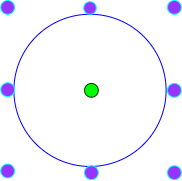
\includegraphics[width=0.2\textwidth]{Immagini/2sensor.png}
        \caption{Neighboors for a sensors are the one immediately adiacent. The purples ones represent the neighboors of green sensor}
        \label{fig:galaxy}
    \end{figure}
    \\
    Defing the range of the sensors equal to their spacing on the grid it follows, depending on agent's position, only a maximum of 4 sensors can be turned on. 
    It follows a figure that show the idea with a 4-sensors grid
    \begin{figure}[h!]
        \centering
        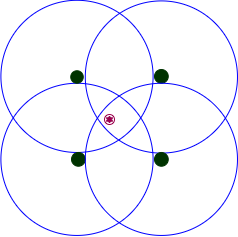
\includegraphics[width=0.23\textwidth]{Immagini/4sensor.png}
        \caption{}
        \label{fig:galaxy}
    \end{figure}
    \begin{itemize}
        \item blue : 1 sensors On 
        \item yellow : 2 sensors On 
        \item orange : 3 sensors On 
        \item red : 4 sensors On 
        \end{itemize}
    % Different state can receive and send different messagesses. A sensor in On state has the moving
    % object in his range and send a CanSense to the nearby and when trackin moving away from the operating range send a CantSense turning itself to Idle.
    % Sensors that receive a CanSense and are not already On turn in Idle state; during the Idle state sensors check
    % if object appears in range sensors turn to On and send a CanSense, if nothing trigger the range it send to the nearby a CantSense signal.
    % A sensor that is in Idle and during the information exchange receive only CantSense from the nearby turn itself Off and stop to check if somenthing is in range and
    % can be turned again to Idle via a CanSense. This scheme implies that a sensors can never switch to On from Off except for the initialization step.
    % \\
    Whenever the target is in range of a sensor, the device takes a measurement at each timestep.
    The model we choose for our measurement device is a radar and as such the measurement function 
    $z(k)=h(x(k))+v(k)$ associated with it is the cartesian to polar transformation, as shown below
    \begin{align*}
        &z(k)=h(x(k))+v(k)\\
        &\begin{bmatrix}
            \rho(k)\\ \alpha(k)
        \end{bmatrix}=  
        \begin{bmatrix}
            \sqrt{x(k)^2+y(k)^2}\\ atan2(y(k)/x(k))
        \end{bmatrix} +
        \begin{bmatrix}
            v_{1}(k)\\v_{2}(k)
        \end{bmatrix}
    \end{align*}
    where $h(x)$ is the polar to cartesian cordinates transform and $v(k)$ is the noise associated to the measurement's operation.

    \begin{equation*}
        \begin{bmatrix}
            \rho\\ \alpha
        \end{bmatrix}=  
        \begin{bmatrix}
            x^2+y^2\\ atan2(y/x)
        \end{bmatrix} 
    \end{equation*}
   for sake of use in the extended Kalman filter, a linearization of $h(x)$ must be performed.
   The LS problem associate becomes
   \begin{equation*}
       x^{SL}(k)=arg min(Z^{k}-h(x)W(Z^{k}-h(x))^{T})= argmin J(x,k)
   \end{equation*}
   and we have to found 
   \begin{equation*}
     \frac{dJ(x,k)}{dx}=0
\end{equation*}
After a bit of management we can compute 
\begin{equation*}
    J(x,k)=Z^{k}
\end{equation*}
        and than it follows that
        \begin{equation*}
            \frac{dJ(x,k)}{dx}=-H(x)^{T}W(Z^{K}-h(x))=0
        \end{equation*}
        where $H(x)=\frac{dh(x)}{dx}$ So in this particular case:
    \begin{equation}
        H= \begin{bmatrix}
            \frac{x}{(x^{2}+y^{2})^{1/2}} & \frac{y}{(x^{2}+y^{2})^{1/2}}& 0& 0 \\
            \frac{-y}{(x^{2}+y^{2})}  & \frac{x}{(x^{2}+y^{2})}& 0& 0 \\
        \end{bmatrix}
    \end{equation}
    \section*{Model used}
    To models the movement of the target has been employed two models: The discrete Wienerprocess acceleration model (DWPA) (reference) and the unicycle model
    Both are Markov process.
    \subsection*{ Discrete Wiener Process Acceleration Model}
    The Discrete Wienerprocess acceleration model choose are described by 5 different mode
    \\
    % \begin{tabular}{ |c|c|c|c|c|c| }
    % \multicolumn{6}{|c|}{Models} \\
    % \begin{tabular}{||c |c  | c  |c|c|c|c|c c c c c||}%{|width=\columnwidth|}
    %     \hline
    %      & DPWA && Unycicle \\
    %     \hline
    %          & Modes & Input & Modes & Inputs\\ [0.5ex]
    %     \hline\hline
    %     state 1 & costant velocity      & $\ddot{x},\ddot{y}=0$ & constant angular velocity &  $\ddot{\omega},\ddot{\alpha}=0$   \\
    %     \hline
    %     state 2  & north acceleration      & $\ddot{x}=\delta$  &  angular acceleration &  $\ddot{\omega}=\delta$ \\
    %     \hline
    %     state 3  & south acceleration    & $\ddot{x}=-\delta$   &  angular deceleration  & $\ddot{\omega}=-\delta$ \\
    %     \hline
    %     state 4  & east acceleration    & $\ddot{y}=\delta$    & acceleration steering (CW) & $\ddot{\omega}=\delta$ \\
    %     \hline
    %     state 5  & west acceleration     & $\ddot{y}=-\delta$  &  acceleration steering (CCW) & $\ddot{\omega}=-\delta$ \\ [1ex]
    %     \hline
    % \end{tabular}
    \begin{center}
    \begin{tabular}{||c||c |c |c| |}%{|width=\columnwidth|}
        \hline
         DPWA  \\
        \hline\hline
         Modes & Description & Input \\ [0.5ex]
        \hline\hline
        mode 1 & costant velocity      & $u(k)=0$    \\
        \hline
        mode 2  & north acceleration      & $u(k)=a $  \\
        \hline
        mode 3  & south acceleration    & $u(k)=-a $   \\
        \hline
        mode 4  & east acceleration    & $u(k)=a $    \\
        \hline
        mode 5  & west acceleration     & $u(k)=-a $   \\ [1ex]
        \hline
    \end{tabular}
\end{center}
    In the case of the DWPA we choosen to have 5 states: costant velocity, positive or negative acceleration
    on x direction and positive or negative deceleration on y direction.
    % \begin{tabular}{||c c c||}%[width=\columnwidth]
    %     \hline
    %     state 1 & costant velocity      & $\ddot{x},\ddot{y}=0$     \\
    %     \hline
    %     state 2  & north acceleration      & $\ddot{x}=\delta$        \\
    %     \hline
    %     state 3  & south acceleration    & $\ddot{x}=-\delta$        \\
    %     \hline
    %     state 4  & east acceleration    & $\ddot{y}=\delta$     \\
    %     \hline
    %     state 5  & west acceleration     & $\ddot{y}=-\delta$       \\ [1ex]
    %     \hline
    % \end{tabular} The Transition matrix 
    % associated with the Markov's chain is shown below
    % \begin{equation*}
    %     \begin{bmatrix}
    %         0.8 & 0.025 & 0.025 & 0.025 & 0.025 //
    %     \end{bmatrix}
    % \end{equation*}
    The linear system describing the evolution of the state is 
    \begin{equation}
        x(k+1)= Ax(k) + B(s)u(k) + Gw(k)
    \end{equation}
    Where $x(k)$ is the state at the current timestep, $u(t)$ is the input and $w(k)$ is the process noise.
    In this case the state is a vector of the cartesian cordinates and their relative speed, while the input 
    is the acceleration which the noise will influence. 
    State,state and noise matrix associate to the DWPA has shown below:
    \[ x=\begin{bmatrix} x \\ y \\ \dot{x} \\ \dot{y} \\ \end{bmatrix}  A=\begin{bmatrix}
            1 & 0 & \delta & 0      \\
            0 & 1 & 0      & \delta \\
            0 & 0 & 1      & 0      \\
            0 & 0 & 0      & 1      \\
        \end{bmatrix}
        G=\begin{bmatrix}
            \delta^2/2 & 0          \\
            0          & \delta^2/2 \\
            \delta     & 0          \\
            0          & \delta     \\
        \end{bmatrix}
    \]
    With $\delta$ time step of the simulation.
    \\
    We hypothesize that the input is unknown in direction but known in magnitude. This set according to the current state at which the markov process is at the timestep.
    This is modeled though the switch between a set of matrices $B(s)$ that change according to the chain's state $s$.
    \begin{equation*}%[width=\columnwidth]
        \resizebox{.9 \columnwidth}{!}{
        $B(s)=\begin{Bmatrix}
            \begin{bmatrix}
                0 & 0 \\
                0          & 0 \\
                0     & 0 \\
                0          & 0 \\
            \end{bmatrix}
            \begin{bmatrix}
                \delta^2/2 & 0 \\
                0          & 0 \\
                \delta     & 0 \\
                0          & 0 \\
            \end{bmatrix}
            \begin{bmatrix}
                -\delta^2/2 & 0 \\
                0          & 0 \\
                -\delta     & 0 \\
                0          & 0 \\
            \end{bmatrix}
            \begin{bmatrix}
                0 & 0          \\
                0 & \delta^2/2 \\
                0 & 0          \\
                0 & \delta     \\
            \end{bmatrix}
            \begin{bmatrix}
                0 & 0          \\
                0 & -\delta^2/2 \\
                0 & 0          \\
                0 & -\delta     \\
            \end{bmatrix}
        \end{Bmatrix} $ 
        }
    \end{equation*}
    \\
    It can be noticed that the matrix $G$ is a merge between the second and the fourth matrices found in the set $B(s)$ as the noise will act
    randomly in direction and magnitude at every time-step.
\subsection*{Unicycle mode}
    The unycicle model has different input and state description. The input are represented by the angular acceleration of the wheel and the steering angle acceleration.
    possible modes are 5: constant angular velocity, acceleration and deceleration of the wheel and positice or negative acceleration of the steering angle.
    \begin{center}
        \resizebox{.99\columnwidth}{!}{ $
        \begin{tabular}{||c||c |c |c| |}%{|width=\columnwidth|}
            \hline
             Unicycle  \\
            \hline\hline
             Modes & & Input \\ [0.5ex]
            \hline\hline
            mode 1 & costant angular velocity      & $u(k)=0$    \\
            \hline
            mode 2  & angular acceleration      & $u(k)=a $  \\
            \hline
            mode 3  & angular deceleration    & $u(k)=-a $   \\
            \hline
            mode 4  & steer angle acceleration (CW)    & $u(k)=a $    \\
            \hline
            mode 5  & steer angle acceleration (CCW)     & $u(k)=-a $   \\ [1ex]
            \hline
        \end{tabular} $}
    \end{center}
    Unycicle model instead is a Non-linear model. The  %Thus is necessary to use a linearization in the Kalman filter implementation
    \begin{equation}
        x(k+1)= Ax(k) + B(s)u(k) + Gw(k)
    \end{equation}
    The matrix that represent the state of system for this case are
    \begin{equation*}      
     \resizebox{.99\columnwidth}{!}{ $ X=\begin{bmatrix} x \\ y \\ \theta \\ \omega \\ \end{bmatrix}  A=\begin{bmatrix}
            1 & 0 & \delta cos(\dot{\theta}) & 0      \\
            0 & 1 & 0      & \delta sin(\dot{\theta}) \\
            0 & 0 & 1      & 0      \\
            0 & 0 & 0      & 1      \\
        \end{bmatrix}
         G=\begin{bmatrix}
            \delta^2/2 cos(\theta)r & 0  \\
            \delta^2/2 sin(\theta)r & 0 \\
            \delta r    & 0          \\
            0 & \delta     \\
        \end{bmatrix}
    $ } \end{equation*}

    We hypothesize that the input is unknown in direction but known in magnitude. This set according to the current state at which the markov process is at the timestep.
    This is modeled though the switch between a set of matrices $B(s)$ that change according to the chain's state $s$.
    \begin{equation*}%[width=\columnwidth]
        \resizebox{.99 \columnwidth}{!}{
        $B(s)=\begin{Bmatrix}
            \begin{bmatrix}
                0 & 0 \\
                0          & 0 \\
                0     & 0 \\
                0          & 0 \\
            \end{bmatrix}
            \begin{bmatrix}
                \delta^2/2 cos(\theta)r & 0 \\
                \delta^2/2 sin(\theta)r & 0 \\
                \delta r    & 0 \\
                0          & 0 \\
            \end{bmatrix}
            \begin{bmatrix}
                -\delta^2/2 cos(\theta)r & 0 \\
                -\delta^2/2 sin(\theta)r & 0 \\
                -\delta r    & 0 \\
                0          & 0 \\
            \end{bmatrix}
            \begin{bmatrix}
                0 & 0          \\
                0 & 0 \\
                0 & 0          \\
                0 & \delta     \\
            \end{bmatrix}
            \begin{bmatrix}
                0 & 0          \\
                0 & 0 \\
                0 & 0          \\
                0 & -\delta     \\
            \end{bmatrix}
        \end{Bmatrix} $ 
        }
    \end{equation*}
    \\
    Also in this case it's possible to notice that $G(s)$ is a merge of $B(s)$
    Therefore in the EKF a linearised model is needed
    and som
    \begin{equation*}
        A(k)
    \end{equation*} 
    \subsection*{Data's simulation}

    \section*{Imm and Linear Consensus}
    In order to reach a more accurate prediction of the trajectory a IMM algorithm is implemented in the sensors's grid. The working principles 
    involves a general knowledge or hypothesis of the model of agent's movement. Every model is used in a Kalman filter stage that use the same measurement and make
    a prediction: the one with the smaller uncertainty is choose as the model for our agent at that timestep. A general scheme of the working principles is shown here (image?)
    \\
    The set of active sensors inside the grid is dynamic, as vertices keep getting added and popped. However it has to be noticed, as stated before, that no 
     more than 4 sensors will be ON at any point of time and they will all be adjacent to each other, this let us model the graph of the active 
     sensors as fully-connected, since the distance between them is short and they are directly linked.
    \\
    \section*{Result}
    The performance evaluation of the system are evaluted by computing the RMS of the predicted trajectory eith the respect to the actual one
    choosing different rate of performind the WSL. The final result are listed in the table below


    \begin{center}
        \begin{tabular}{||c c c c||}
            \hline
            1 step & 2 step & 3 step & 4 step \\ [0.5ex]
            \hline\hline
            1      & 6      & 87837  & 787    \\
            \hline
            2      & 7      & 78     & 5415   \\
            \hline
            3      & 545    & 778    & 7507   \\
            \hline
            4      & 545    & 18744  & 7560   \\
            \hline
            5      & 88     & 788    & 6344   \\ [1ex]
            \hline
        \end{tabular}
    \end{center}


    \subsection*{tabelle}

    
    \begin{center}
        \resizebox{.99\columnwidth}{!}{ $
        \begin{tabular}{||c||c |c |c|c| |}%{|width=\columnwidth|}
            \hline
             Consensus rate 20  \\
            \hline\hline
              & Mean of Imm's mean & Max of Imm's mean & max of IMM's max  \\ [0.5ex]
            \hline\hline
            R1,Q1  & costant angular velocity      & $u(k)=0$    \\
            \hline
            R1,Q2   & angular acceleration      & $u(k)=a $  \\
            \hline
            R2,Q1   & angular deceleration    & $u(k)=-a $   \\
            \hline
            R2,Q2  & steer angle acceleration (CW)    & $u(k)=a $    \\
            \hline
           
        \end{tabular} 
        \\
        \begin{tabular}{||c||c |c |c|c| |}%{|width=\columnwidth|}
            \hline
             Consensus rate 20  \\
            \hline\hline
              & Mean of Imm's mean & Max of Imm's mean & max of IMM's max  \\ [0.5ex]
            \hline\hline
            R1,Q1  & costant angular velocity      & $u(k)=0$    \\
            \hline
            R1,Q2   & angular acceleration      & $u(k)=a $  \\
            \hline
            R2,Q1   & angular deceleration    & $u(k)=-a $   \\
            \hline
            R2,Q2  & steer angle acceleration (CW)    & $u(k)=a $    \\
            \hline
           
        \end{tabular} $}
    \end{center}

    
    \begin{center}
        \resizebox{.99\columnwidth}{!}{ $
        \begin{tabular}{||c||c |c |c|c| |}%{|width=\columnwidth|}
            \hline
             Consensus rate 20  \\
            \hline\hline
              & Mean of Imm's mean & Max of Imm's mean & max of IMM's max  \\ [0.5ex]
            \hline\hline
            R1,Q1  & costant angular velocity      & $u(k)=0$    \\
            \hline
            R1,Q2   & angular acceleration      & $u(k)=a $  \\
            \hline
            R2,Q1   & angular deceleration    & $u(k)=-a $   \\
            \hline
            R2,Q2  & steer angle acceleration (CW)    & $u(k)=a $    \\
            \hline
           
        \end{tabular} $}
    \end{center}


\end{document}
